
\subsection{M�todos}

A partir das limpeza dos dados, para an�lise de ambos datasets gerados, lan�ou-se m�o de m�todos cl�ssicos do \textit{Machine learning} sendo eles: Regress�o log�stica, Naive Bayes, Florestas Aleat�rias e \textit{XGBoost}. Al�m deles, para compara��o, utilizou-se uma rede neural artificial LSTM. Esses m�todos ser�o aqui melhor detalhados.

% Regress�o log�stica

\subsubsection{Regress�o Log�stica}

A regress�o log�stica � um modelo estat�stico robusto e eficiente, que permite a previs�o da probabilidade de um evento bin�rio de forma precisa e confi�vel \citep{hosmer2013applied}. Este tipo de evento � aquele que pode ocorrer ou n�o, ou que pode ser classificado em duas categorias distintas. Por exemplo, em uma an�lise de cr�dito, o cliente pode ser aprovado ou n�o. Na medicina, o evento pode ser a cura ou n�o de uma doen�a.

Ela apresenta um modelo linear generalizado que utiliza a fun��o log�stica para modelar a rela��o entre as vari�veis independentes e a vari�vel dependente \citep{kleinbaum2010logistic}. A fun��o log�stica � uma fun��o sigmoide que transforma uma vari�vel linear em uma probabilidade. A equa��o da fun��o log�stica � dada por:

\begin{equation}
    p = \frac{1}{1 + e^{-x}}
\end{equation}

Sendo $p$ a probabilidade do evento ocorrer, $x$ uma vari�vel linear que representa a combina��o linear das vari�veis independentes, e $e$ a constante de Euler.

A regress�o log�stica utiliza a t�cnica de m�xima verossimilhan�a para estimar os par�metros do modelo a partir dos dados observados. A fun��o de verossimilhan�a � maximizada para encontrar os valores dos coeficientes que melhor se ajustam aos dados. O modelo � ajustado para minimizar a diferen�a entre as probabilidades previstas pelo modelo e as probabilidades observadas nos dados \citep{mccullagh1989generalized}.

A regress�o log�stica tem sido amplamente utilizada em diversas �reas, como na an�lise de dados de sobreviv�ncia, na an�lise de dados de sa�de, na an�lise de dados financeiros, etc. Por exemplo, � utilizada na an�lise de dados de sobreviv�ncia para modelar a probabilidade de um paciente sobreviver a uma doen�a com base em fatores como idade, sexo, n�vel de educa��o, etc. Na an�lise de dados financeiros, � utilizada para modelar a probabilidade de um cliente pagar ou n�o uma d�vida com base em fatores como hist�rico de cr�dito, renda, etc.


\begin{figure}[H]
    \centering
    \begin{tikzpicture}
        \begin{axis}[    axis lines=left,    xlabel=$x$,    ylabel=$y$,    ymin=0, ymax=1,    ytick={0,1},    xmin=-5, xmax=5,    legend pos=north west]
            \addplot[domain=-5:5, samples=100, blue, thick] {1/(1+exp(-x))};
            \addlegendentry{$\frac{1}{1+e^{-x}}$};
            \draw[dashed] (axis cs:-5,0.5) -- (axis cs:5,0.5);
            \addplot[only marks, mark=*, red] coordinates {
                    (-4, 0.1)
                    (-1, 0.3)
                    (0, 0.6)
                    (1, 0.8)
                    (2, 0.9)
                    (4, 0.96)
                };
            \addlegendentry{Dados}
        \end{axis}
    \end{tikzpicture}
    \caption{Modelo gráfico da regressão logística (curva sigmoide)}
    \label{plt:logistic}
\end{figure}

% Classifica��o Naive Bayes

\subsubsection{Naive Bayes}

A classifica��o Naive Bayes � um algoritmo de aprendizado de m�quina supervisionado que utiliza o teorema de Bayes para classificar inst�ncias em classes discretas. A principal vantagem do algoritmo Naive Bayes � a sua simplicidade e efici�ncia computacional, o que o torna uma escolha popular para problemas de classifica��o em grande escala \citep{mitchell1997machine}.

O algoritmo Naive Bayes � baseado no teorema de Bayes, que fornece uma maneira de calcular a probabilidade condicional de uma hip�tese, dado um conjunto de evid�ncias. Na classifica��o, a hip�tese corresponde � classe da inst�ncia e as evid�ncias correspondem �s caracter�sticas observadas da inst�ncia. O algoritmo calcula a probabilidade condicional de cada classe, dado as caracter�sticas observadas da inst�ncia, e atribui a inst�ncia � classe com a maior probabilidade condicional.

Segundo \cite{domingos1997optimality}, a principal suposi��o por tr�s do algoritmo Naive Bayes � a independ�ncia condicional das caracter�sticas, ou seja, cada caracter�stica contribui independentemente para a probabilidade condicional de cada classe. Embora essa suposi��o seja muitas vezes violada na pr�tica, o algoritmo Naive Bayes ainda funciona bem em muitos casos e pode ser especialmente �til quando h� muitas caracter�sticas.

O algoritmo Naive Bayes tem sido aplicado em muitas �reas, incluindo reconhecimento de fala, processamento de texto e detec��o de spam de e-mail. � particularmente �til em aplica��es onde h� muitas caracter�sticas e as inst�ncias s�o discretas ou categ�ricas. Um estudo emp�rico sobre o desempenho do algoritmo Naive Bayes em diferentes conjuntos de dados pode ser encontrado em \citep{rish2001empirical}.

Embora o algoritmo Naive Bayes seja uma t�cnica de classifica��o simples e eficiente, ele tamb�m tem algumas limita��es. Por exemplo, a suposi��o de independ�ncia condicional das caracter�sticas pode ser inadequada em algumas situa��es, e a performance do algoritmo pode ser afetada por dados ausentes ou dados ruidosos \citep{mitchell1997machine}.

As equa��es abaixo representam a base matem�tica do algoritmo de classifica��o Naive Bayes:

Dada uma inst�ncia $X = {x_1, x_2, \dots, x_n}$ com caracter�sticas observadas, o objetivo do algoritmo � determinar a probabilidade condicional $P(C_k|X)$ da inst�ncia pertencer a cada classe $C_k$.

O teorema de Bayes fornece uma maneira de calcular a probabilidade condicional $P(C_k|X)$ em termos das probabilidades a priori $P(C_k)$ e das probabilidades condicionais $P(X|C_k)$, como segue:

\begin{equation}
    P(C_k|X)=\frac{P(X|C_k)P(C_k)}{P(X)}
\end{equation}

Aqui, $P(C_k)$ � a probabilidade a priori da classe $C_k$ e $P(X|C_k)$ � a probabilidade condicional de observar a inst�ncia $X$ dada a classe $C_k$.

O classificador Naive Bayes assume a independ�ncia condicional das caracter�sticas dadas a classe, isto �, $P(x_i|C_k, x_1, \dots, x_{i-1}, x_{i+1}, \dots, x_n) = P(x_i|C_k)$. Isso permite simplificar a probabilidade condicional $P(X|C_k)$ como:

\begin{equation}
    P(X|C_k)=P(x_1, \dots, x_{i-1}, x_{i+1}, \dots, x_n|C_k)=\prod_{i=1}^{n}P(x_i|C_k)
\end{equation}

Substituindo essa express�o na equa��o anterior, tem-se:

\begin{equation}
    P(C_k|X)=\frac{\prod_{i=1}^{n}P(x_i|C_k)P(C_k)}{P(X)}
\end{equation}

Como a probabilidade $P(X)$ � constante para todas as classes, � poss�vel comparar apenas as probabilidades $P(C_k)\prod_{i=1}^n P(x_i|C_k)$ para determinar a classe mais prov�vel para a inst�ncia $X$.

O desenho ilustra as vari�veis aleat�rias $x_1, x_2, x_3, x_4$ e a classe $C_k$. As setas que partem das probabilidades condicionais e a priori indicam as f�rmulas para o c�lculo das probabilidades conjuntas $P(x_1, x_2, x_3, x_4, C_k)$ e, consequentemente, para a classifica��o de uma inst�ncia.

\begin{figure}[H]
    \centering
    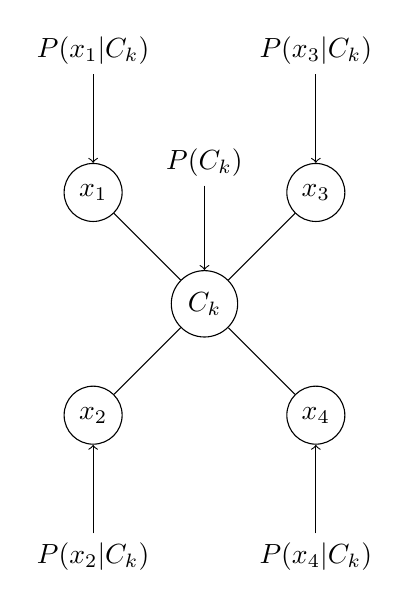
\begin{tikzpicture}[node distance=2cm, auto]
        % Define os nós
        \node[draw, circle] (C) {$C_k$};
        \node[draw, circle, above left of=C] (X1) {$x_1$};
        \node[draw, circle, below left of=C] (X2) {$x_2$};
        \node[draw, circle, above right of=C] (X3) {$x_3$};
        \node[draw, circle, below right of=C] (X4) {$x_4$};
        % Conecta os nós
        \draw[-] (X1) -- (C);
        \draw[-] (X2) -- (C);
        \draw[-] (X3) -- (C);
        \draw[-] (X4) -- (C);
        % Adiciona as probabilidades condicionais
        \node[above of=X1, yshift=-0.2cm] (px1ck) {$P(x_1|C_k)$};
        \node[below of=X2, yshift=0.2cm] (px2ck) {$P(x_2|C_k)$};
        \node[above of=X3, yshift=-0.2cm] (px3ck) {$P(x_3|C_k)$};
        \node[below of=X4, yshift=0.2cm] (px4ck) {$P(x_4|C_k)$};
        % Adiciona as probabilidades a priori
        \node[above of=C, yshift=-0.2cm] (pck) {$P(C_k)$};
        % Adiciona as setas com as fórmulas
        \draw[->] (pck) -- (C);
        \draw[->] (px1ck) -- (X1);
        \draw[->] (px2ck) -- (X2);
        \draw[->] (px3ck) -- (X3);
        \draw[->] (px4ck) -- (X4);
    \end{tikzpicture}
    \caption{Esquema de funcionamento da classificação Naive Bayes}
    \label{plt:bayes}
\end{figure}

% Florestas aleat�rias

\subsubsection{Florestas aleat�rias}

De acordo com \cite{breiman2001random}, as florestas aleat�rias s�o uma t�cnica de aprendizado de m�quina que combina v�rias �rvores de decis�o para construir um modelo de classifica��o ou regress�o. Cada �rvore de decis�o � constru�da a partir de um subconjunto aleat�rio dos dados de treinamento e um subconjunto aleat�rio dos recursos (tamb�m conhecidos como caracter�sticas ou atributos). Esses subconjuntos s�o criados para garantir que cada �rvore de decis�o seja diferente e que a floresta aleat�ria possa capturar v�rias rela��es entre os dados e recursos.

A constru��o de uma �rvore de decis�o � feita por meio de uma s�rie de etapas. Inicialmente, a �rvore come�a com um �nico n� que representa todo o conjunto de dados de treinamento. Em seguida, a �rvore � dividida em n�s menores usando uma fun��o de divis�o que escolhe um recurso e um ponto de divis�o que minimiza a impureza dos dados. A impureza � uma medida da desorganiza��o dos dados, que pode ser medida por diferentes crit�rios, como a entropia ou o �ndice Gini. O processo de divis�o � repetido recursivamente at� que os n�s finais sejam puros ou um crit�rio de parada seja atingido, como uma profundidade m�xima da �rvore \citep{cutler2001random}.

Durante a fase de teste, a floresta aleat�ria retorna a classe mais comum ou a m�dia das sa�das das �rvores individuais, dependendo se o problema � de classifica��o ou regress�o, respectivamente.

As florestas aleat�rias apresentam v�rias vantagens em rela��o a outras t�cnicas de aprendizado de m�quina. Em primeiro lugar, elas t�m um bom desempenho em dados de alta dimens�o, onde o n�mero de recursos � grande em rela��o ao n�mero de amostras. Em segundo lugar, elas s�o relativamente insens�veis a outliers e dados ausentes. Em terceiro lugar, elas s�o facilmente paraleliz�veis, permitindo que grandes conjuntos de dados sejam processados em paralelo em clusters de computadores \citep{cutler2001random}.

Em termos de aplica��o, elas s�o amplamente utilizadas em uma variedade de problemas, como reconhecimento de padr�es em imagens e sinais, detec��o de fraudes em transa��es financeiras, an�lise de sentimentos em redes sociais, previs�o de pre�os de a��es e an�lise de dados gen�micos \citep{breiman2001random}.

As equa��es relacionadas �s florestas aleat�rias s�o principalmente as usadas na constru��o de cada �rvore de decis�o. Por exemplo, as equa��es para o c�lculo da impureza dos dados, que � um dos principais crit�rios de divis�o de n�s em uma �rvore de decis�o s�o dadas:

\begin{itemize}
    \item O �ndice Gini:
          \begin{equation}
              G_i = \sum_{k=1}^{K} p_{i,k} (1-p_{i,k}),
          \end{equation}

          onde $K$ � o n�mero de classes, $p_{i,k}$ � a propor��o de observa��es da classe $k$ no n� $i$.
    \item A entropia:
          \begin{equation}
              H_i = -\sum_{k=1}^{K} p_{i,k} \log(p_{i,k}),
          \end{equation}

          onde $K$ � o n�mero de classes, $p_{i,k}$ � a propor��o de observa��es da classe $k$ no n� $i$.

    \item O crit�rio de divis�o de Gini � dado por:
          \begin{equation}
              G_{d} = \sum_{i=1}^{q}\frac{n_i}{n}G_i,
          \end{equation}

          onde $q$ � o n�mero de n�s filhos resultantes da divis�o, $n_i$ � o n�mero de observa��es no n� $i$ e $n$ � o n�mero total de observa��es.

    \item O crit�rio de divis�o de entropia � dado por:
          \begin{equation}
              H_{d} = -\sum_{i=1}^{q}\frac{n_i}{n}H_i,
          \end{equation}

          onde $q$ � o n�mero de n�s filhos resultantes da divis�o, $n_i$ � o n�mero de observa��es no n� $i$ e $n$ � o n�mero total de observa��es.

\end{itemize}

Essas equa��es s�o usadas para calcular a impureza dos dados em cada n� da �rvore de decis�o e, assim, decidir qual recurso e ponto de divis�o usar para dividir o n� em dois filhos. O processo de divis�o � repetido recursivamente para construir a �rvore de decis�o completa. Em seguida, v�rias �rvores de decis�o s�o combinadas para formar a floresta aleat�ria.



\usetikzlibrary{fit,shapes.arrows,positioning}

\tikzset{marrow/.style={midway,red,sloped,fill, minimum height=3cm, single arrow, single arrow
            head extend=.5cm, single arrow head indent=.25cm,xscale=0.3,yscale=0.15,
            allow upside down}}
\begin{figure}[H]
    \centering
    \scalebox{0.48}{
        \begin{forest}
            for tree={l sep=3em, s sep=3em, anchor=center, inner sep=0.7em, fill=blue!50,
            circle, font=\Large\sffamily,where level=1{no edge}{}}
            [Dados de treinamento, draw, rectangle, rounded corners, orange, text=white,alias=TD
            [,red!70,alias=a1[[,alias=a2][]][,red!70,edge label={node[above=1ex,marrow]{}}[[][]][,red!70,edge label={node[above=1ex,marrow]{}}[,red!70,edge label={node[below=1ex,marrow]{}}][,alias=a3]]]]
            [,red!70,alias=b1[,red!70,edge label={node[below=1ex,marrow]{}}[[,alias=b2][]][,red!70,edge label={node[above=1ex,marrow]{}}]][[][[][,alias=b3]]]]
            [~$\cdots$~,scale=4,no edge,fill=none,yshift=-1em]
            [,red!70,alias=c1[[,alias=c2][]][,red!70,edge label={node[above=1ex,marrow]{}}[,red!70,edge label={node[above=1ex,marrow]{}}[,alias=c3][,red!70,edge label={node[above=1ex,marrow]{}}]][,alias=c4]]]
            ]
            \node[draw,fit=(a1)(a2)(a3)](f1){};
            \node[draw,fit=(b1)(b2)(b3)](f2){};
            \node[draw,fit=(c1)(c2)(c3)(c4)](f3){};
            \path (f1.south west)--(f3.south east) node[midway,below=4em] (D) {Média};
            \node[below=2em of D] (pred){Predição};
            \foreach \X in {1,2,3}{\draw[-stealth] (TD) -- (f\X.north);
                    \draw[-stealth] (f\X.south) -- (D);}
            \draw[-stealth] (D) -- (pred);
        \end{forest}
    }
    \caption{Esquema de funcionamento de uma floresta aleatória}
    \label{plt:randomForest}
\end{figure}











% XGBoost

\subsubsection{XGBoost}

O XGBoost (\textit{Extreme Gradient Boosting}) � um m�todo de aprendizado de m�quina baseado em �rvores de decis�o, assim como as florestas aleat�rias, mas com algumas diferen�as importantes. Enquanto as florestas aleat�rias usam um conjunto de �rvores de decis�o independentes para fazer uma previs�o, o XGBoost usa um conjunto de �rvores de decis�o sequenciais que s�o criadas iterativamente. Cada nova �rvore � ajustada aos res�duos do modelo anterior, tentando corrigir os erros cometidos pelo modelo atual.

O algoritmo XGBoost foi desenvolvido por Tianqi Chen e Carlos Guestrin em 2016 \citep{Chen:2016} e � baseado na biblioteca de c�digo aberto de mesmo nome. O XGBoost se tornou um dos algoritmos de aprendizado de m�quina mais populares em competi��es de ci�ncia de dados e � amplamente utilizado na ind�stria.

O processo de constru��o do modelo XGBoost pode ser descrito por meio da seguinte equa��o:

\begin{equation}
    \hat{y_i} = \phi(\mathbf{x}_i) = \sum_{k=1}^{K}(\mathbf{x}_i)
\end{equation}

onde $\hat{y_i}$ � a previs�o para a i-�sima inst�ncia, $\phi$ � a fun��o de previs�o, $\mathbf{x}_i$ � o vetor de caracter�sticas para a i-�sima inst�ncia, $K$ � o n�mero total de �rvores no modelo e $f_k$ � a k-�sima �rvore de decis�o.

Para construir o modelo XGBoost, o algoritmo usa um processo iterativo de adi��o de �rvores, onde cada nova �rvore � ajustada aos res�duos do modelo anterior, tentando corrigir os erros cometidos pelo modelo atual. Esse processo � descrito pela seguinte equa��o:

\begin{equation}
    \mathbf{F}_k = \mathbf{F}_{k-1} + \gamma_k f_k
\end{equation}

onde $\mathbf{F}_k$ � a soma cumulativa das previs�es das �rvores anteriores at� a k-�sima �rvore, $\gamma_k$ � a taxa de aprendizado da k-�sima �rvore e $f_k$ � a k-�sima �rvore de decis�o.

O XGBoost tamb�m usa um conjunto de hiperpar�metros para ajustar o modelo e evitar overfitting. Alguns dos hiperpar�metros mais importantes incluem:

\begin{itemize}
    \item N�mero de �rvores: o n�mero total de �rvores a serem criadas;
    \item Profundidade m�xima: o n�mero m�ximo de camadas que cada �rvore pode ter;
    \item Taxa de aprendizado: a taxa na qual o modelo tenta corrigir os erros cometidos pelas �rvores anteriores;
    \item Subamostragem: a fra��o de amostras de treinamento a serem usadas para treinar cada �rvore;
    \item Colsample: a fra��o de recursos (caracter�sticas) a serem amostrados aleatoriamente para cada �rvore.
\end{itemize}

Chen e Guestrin descrevem o algoritmo XGBoost em detalhes em seu artigo "XGBoost: A Scalable Tree Boosting System" \citep{Chen:2016}, onde eles mostram que o XGBoost pode superar outros algoritmos de aprendizado de m�quina em uma variedade de conjuntos de dados e tarefas.

Uma das principais vantagens do XGBoost � sua efici�ncia computacional. O algoritmo usa v�rias t�cnicas para reduzir o tempo de treinamento e a complexidade do modelo, incluindo a amostragem de caracter�sticas, a paraleliza��o do processo de treinamento e o uso de uma estrutura de dados espec�fica chamada "gradiente e Hessiano".

O XGBoost � amplamente utilizado em competi��es de ci�ncia de dados e em projetos de aprendizado de m�quina na ind�stria. A biblioteca XGBoost � de c�digo aberto e est� dispon�vel para v�rias linguagens de programa��o, incluindo Python, R e Java.

As seguintes equa��es s�o usadas para calcular os valores dos gradientes e Hessiano para cada inst�ncia $i$:

\begin{equation}
    \begin{aligned}
         & g_i = \frac{\partial L (y_i, \hat{y_i})}{\partial \hat{y_i}},      \\
         & h_i = \frac{\partial^2 L (y_i, \hat{y_i})}{\partial \hat{y_{i}}^2}
    \end{aligned}
\end{equation}


onde $L$ � a fun��o de perda usada para avaliar a qualidade da previs�o. O XGBoost usa esses valores de gradiente e Hessiano para ajustar as �rvores do modelo, tentando minimizar a fun��o de perda.

% Redes Neurais

\subsubsection{Redes Neurais}

\def\layersep{2.5cm}

\begin{figure}[H]
    \centering
    \scalebox{1.5}{
        \begin{tikzpicture}[shorten >=1pt,->,draw=black!50, node distance=\layersep]
            \tikzstyle{every pin edge}=[<-,shorten <=1pt]
            \tikzstyle{neuron}=[circle,fill=black!25,minimum size=17pt,inner sep=0pt]
            \tikzstyle{input neuron}=[neuron, fill=green!50];
            \tikzstyle{output neuron}=[neuron, fill=red!50];
            \tikzstyle{hidden neuron}=[neuron, fill=blue!50];
            \tikzstyle{annot} = [text width=4em, text centered]

            % Draw the input layer nodes
            \foreach \name / \y in {1,...,4}
            % This is the same as writing \foreach \name / \y in {1/1,2/2,3/3,4/4}
            \node[input neuron, pin=left:Input \#\y] (I-\name) at (0,-\y) {};

            % Draw the hidden layer nodes
            \foreach \name / \y in {1,...,5}
            \path[yshift=0.5cm]
            node[hidden neuron] (H-\name) at (\layersep,-\y cm) {};

            % Draw the output layer node
            \node[output neuron,pin={[pin edge={->}]right:Output}, right of=H-3] (O) {};

            % Connect every node in the input layer with every node in the
            % hidden layer.
            \foreach \source in {1,...,4}
            \foreach \dest in {1,...,5}
            \path (I-\source) edge (H-\dest);

            % Connect every node in the hidden layer with the output layer
            \foreach \source in {1,...,5}
            \path (H-\source) edge (O);

            % Annotate the layers
            \node[annot,above of=H-1, node distance=1cm] (hl) {Camada escondida};
            \node[annot,left of=hl] {Camada de entrada};
            \node[annot,right of=hl] {Camada de sa�da};
        \end{tikzpicture}
    }
    \caption{Esquema simples de funcionamento de uma rede neural}
    \label{plt:neural}
\end{figure}

Redes Neurais Artificiais (RNAs) s�o modelos computacionais que se inspiram no funcionamento do c�rebro humano e t�m sido amplamente utilizadas para tarefas de classifica��o, previs�o e reconhecimento de padr�es em diferentes �reas do conhecimento. O conceito de RNA foi proposto por \cite{mcculloch1943logical}, mas foi apenas a partir da d�cada de 1980, com o desenvolvimento de t�cnicas de treinamento de redes profundas, que as RNAs se tornaram uma ferramenta poderosa para an�lise de dados \cite{lecun2015deep}.

Uma RNA � composta por camadas de neur�nios artificiais, cada um com uma fun��o de ativa��o que transforma a entrada recebida em uma sa�da. A primeira camada � a camada de entrada, que recebe os dados a serem processados. A �ltima camada � a camada de sa�da, que produz a resposta final da RNA. Entre as camadas de entrada e sa�da, podem ser adicionadas v�rias camadas ocultas, que ajudam a extrair caracter�sticas dos dados de entrada.

O processo de treinamento de uma RNA consiste em ajustar os pesos sin�pticos entre os neur�nios para que a rede produza a sa�da correta para cada entrada. O algoritmo mais comum de treinamento � o Backpropagation, proposto por \cite{rumelhart1986parallel}. O Backpropagation utiliza o m�todo do gradiente descendente para minimizar a fun��o de custo da RNA em rela��o aos pesos sin�pticos.

Uma das principais vantagens das RNAs � a capacidade de lidar com dados complexos e n�o lineares. Al�m disso, as RNAs podem ser utilizadas em problemas de classifica��o, previs�o e reconhecimento de padr�es em diferentes �reas, como vis�o computacional, processamento de fala, processamento de texto e bioinform�tica.

No entanto, as RNAs possuem algumas desvantagens, como a dificuldade de interpreta��o dos resultados e o risco de overfitting, que ocorre quando a rede se ajusta demais aos dados de treinamento e n�o consegue generalizar para novos dados.

As redes neurais artificiais s�o compostas por uma s�rie de camadas de neur�nios, que realizam opera��es matem�ticas nas entradas recebidas para gerar sa�das. A formula��o matem�tica dessas opera��es pode variar de acordo com a arquitetura da rede, mas em geral envolvem uma combina��o linear das entradas, seguida de uma fun��o n�o linear de ativa��o.

Abaixo tem-se as equa��es matem�ticas para uma rede neural \textit{feedforward} de tr�s camadas, com $n^{(l)}$ neur�nios na camada $l$:

\begin{equation}
    \begin{aligned}
         & z_j^{(2)} = \sum\limits_{i=1}^{n^{(1)}} w_{ij}^{(1)} x_i + b_j^{(1)}       \\
         & h_j^{(2)} = f(z_j^{(2)})                                                   \\
         & z_k^{(3)} = \sum\limits_{j=1}^{n^{(2)}} w_{jk}^{(2)} h_j^{(2)} + b_k^{(2)} \\
         & y_k = f(z_k^{(3)})
    \end{aligned}
\end{equation}

Na equa��o acima, $x_i$ representa a entrada na posi��o $i$, $w_{ij}^{(1)}$ representa o peso associado � conex�o entre o neur�nio $i$ da camada de entrada e o neur�nio $j$ da camada oculta, $b_j^{(1)}$ � o vi�s associado ao neur�nio $j$ da camada oculta, $f$ � a fun��o de ativa��o, $h_j^{(2)}$ � a sa�da do neur�nio $j$ da camada oculta, $w_{jk}^{(2)}$ � o peso associado � conex�o entre o neur�nio $j$ da camada oculta e o neur�nio $k$ da camada de sa�da, $b_k^{(2)}$ � o vi�s associado ao neur�nio $k$ da camada de sa�da e $y_k$ � a sa�da final da rede neural.

� importante notar que a escolha da fun��o de ativa��o pode influenciar significativamente o comportamento da rede neural, permitindo, por exemplo, que ela aprenda a modelar fun��es n�o-lineares complexas. Algumas fun��es de ativa��o comuns incluem a fun��o sigmoide, a fun��o tangente hiperb�lica e a fun��o ReLU (Rectified Linear Unit).

